% Options for packages loaded elsewhere
\PassOptionsToPackage{unicode}{hyperref}
\PassOptionsToPackage{hyphens}{url}
%
\documentclass[
  11pt,
]{article}
\usepackage{amsmath,amssymb}
\usepackage{iftex}
\ifPDFTeX
  \usepackage[T1]{fontenc}
  \usepackage[utf8]{inputenc}
  \usepackage{textcomp} % provide euro and other symbols
\else % if luatex or xetex
  \usepackage{unicode-math} % this also loads fontspec
  \defaultfontfeatures{Scale=MatchLowercase}
  \defaultfontfeatures[\rmfamily]{Ligatures=TeX,Scale=1}
\fi
\usepackage{lmodern}
\ifPDFTeX\else
  % xetex/luatex font selection
\fi
% Use upquote if available, for straight quotes in verbatim environments
\IfFileExists{upquote.sty}{\usepackage{upquote}}{}
\IfFileExists{microtype.sty}{% use microtype if available
  \usepackage[]{microtype}
  \UseMicrotypeSet[protrusion]{basicmath} % disable protrusion for tt fonts
}{}
\makeatletter
\@ifundefined{KOMAClassName}{% if non-KOMA class
  \IfFileExists{parskip.sty}{%
    \usepackage{parskip}
  }{% else
    \setlength{\parindent}{0pt}
    \setlength{\parskip}{6pt plus 2pt minus 1pt}}
}{% if KOMA class
  \KOMAoptions{parskip=half}}
\makeatother
\usepackage{xcolor}
\usepackage[left = 2.5cm, right = 2cm, top = 2cm, bottom =
2cm]{geometry}
\usepackage{longtable,booktabs,array}
\usepackage{calc} % for calculating minipage widths
% Correct order of tables after \paragraph or \subparagraph
\usepackage{etoolbox}
\makeatletter
\patchcmd\longtable{\par}{\if@noskipsec\mbox{}\fi\par}{}{}
\makeatother
% Allow footnotes in longtable head/foot
\IfFileExists{footnotehyper.sty}{\usepackage{footnotehyper}}{\usepackage{footnote}}
\makesavenoteenv{longtable}
\usepackage{graphicx}
\makeatletter
\def\maxwidth{\ifdim\Gin@nat@width>\linewidth\linewidth\else\Gin@nat@width\fi}
\def\maxheight{\ifdim\Gin@nat@height>\textheight\textheight\else\Gin@nat@height\fi}
\makeatother
% Scale images if necessary, so that they will not overflow the page
% margins by default, and it is still possible to overwrite the defaults
% using explicit options in \includegraphics[width, height, ...]{}
\setkeys{Gin}{width=\maxwidth,height=\maxheight,keepaspectratio}
% Set default figure placement to htbp
\makeatletter
\def\fps@figure{htbp}
\makeatother
\setlength{\emergencystretch}{3em} % prevent overfull lines
\providecommand{\tightlist}{%
  \setlength{\itemsep}{0pt}\setlength{\parskip}{0pt}}
\setcounter{secnumdepth}{5}
\usepackage{float}
\usepackage{sectsty}
\usepackage{paralist}
\usepackage{setspace}\spacing{1.0}
\usepackage{fancyhdr}
\usepackage{lastpage}
\usepackage{dcolumn}
\usepackage{natbib}\bibliographystyle{agsm}
\usepackage[nottoc, numbib]{tocbibind}
\ifLuaTeX
  \usepackage{selnolig}  % disable illegal ligatures
\fi
\usepackage{bookmark}
\IfFileExists{xurl.sty}{\usepackage{xurl}}{} % add URL line breaks if available
\urlstyle{same}
\hypersetup{
  hidelinks,
  pdfcreator={LaTeX via pandoc}}

\author{}
\date{\vspace{-2.5em}}

\begin{document}

\subsectionfont{\raggedright}
\subsubsectionfont{\raggedright}

\pagenumbering{gobble}

\begin{centering}

\vspace{3cm}


\begin{center}\includegraphics[width=0.8\linewidth,height=0.8\textwidth]{../../../Users/jaimem/University of Tasmania/IMAS - Documents/Approved Logos/UniTas_IMAS_P_Pos_Col_RGB_2021} \end{center}

\vspace{4cm}

\LARGE

\doublespacing
{\bf Examining the role of size limits in determining catch composition using length-weight commercial abalone catch sampling data}

\vspace{4 cm}

\Large
{\bf Institute for Marine and Antarctic Studies}

\Large
{\bf Univeristy of Tasmania}

\vspace{1cm}

\normalsize
\singlespacing
By

\vspace{0.5 cm}

\large

{\bf Jaime McAllister}

\vspace{1.5 cm}

\normalsize
June 2024

\end{centering}

\newpage

\section{Background}\label{background}

Harvest Strategy and movement towards SAM + 3-years growth (3-year rule)
- traditionally been 2-year rule.

Scheduled LML increase - 138 to 140 mm in 2023, 140 to 142 in 2024, and
142 to 145 in 2025.

Argument that some populations do not reach the sizes proposed in the
scheduled, and LML increases will reduce CPUE and trigger catch
reduction under MCDA settings of harvest strategy.

Here we explore the effects of increasing size limits on the commercial
abalone fishery harvest in Tasmania's Eastern Zone.

\section{Commercial catch sampling
data}\label{commercial-catch-sampling-data}

\begin{center}\includegraphics[width=0.8\textwidth,height=0.8\textwidth]{MM_Length-Weight_LML_files/figure-latex/lwplot check-1} \end{center}

\begin{center}\includegraphics[width=0.8\textwidth,height=0.8\textwidth]{MM_Length-Weight_LML_files/figure-latex/lw clean plot-1} \end{center}

\begin{longtable}[]{@{}rlrrrr@{}}
\caption{Summary of catches measured from commerical abalone catch
sampling data for EZ Blocks collected between 2019-2024.}\tabularnewline
\toprule\noalign{}
FishingYear & BlockNo & Catches & n & Mean Length & Mean Weight \\
\midrule\noalign{}
\endfirsthead
\toprule\noalign{}
FishingYear & BlockNo & Catches & n & Mean Length & Mean Weight \\
\midrule\noalign{}
\endhead
\bottomrule\noalign{}
\endlastfoot
2019 & 13 & 10 & 911 & 146 & 509 \\
2019 & 14 & 1 & 97 & 157 & 683 \\
2019 & 16 & 1 & 92 & 150 & 588 \\
2019 & 21 & 1 & 94 & 151 & 591 \\
2020 & 13 & 45 & 3961 & 148 & 564 \\
2020 & 14 & 7 & 570 & 152 & 591 \\
2020 & 20 & 5 & 405 & 150 & 583 \\
2020 & 21 & 7 & 667 & 153 & 601 \\
2020 & 29 & 1 & 92 & 147 & 528 \\
2020 & 31 & 2 & 173 & 147 & 599 \\
2021 & 13 & 83 & 7998 & 149 & 550 \\
2021 & 14 & 12 & 1164 & 151 & 577 \\
2021 & 17 & 1 & 19 & 151 & 623 \\
2021 & 20 & 5 & 483 & 149 & 571 \\
2021 & 21 & 12 & 1159 & 153 & 584 \\
2021 & 29 & 1 & 98 & 150 & 568 \\
2022 & 13 & 96 & 9235 & 147 & 551 \\
2022 & 14 & 16 & 1537 & 151 & 592 \\
2022 & 20 & 5 & 469 & 151 & 588 \\
2022 & 21 & 16 & 1528 & 154 & 596 \\
2023 & 13 & 40 & 3758 & 150 & 582 \\
2023 & 14 & 2 & 189 & 154 & 631 \\
2023 & 20 & 2 & 194 & 151 & 616 \\
2023 & 21 & 7 & 702 & 156 & 624 \\
2023 & 29 & 1 & 100 & 154 & 591 \\
\end{longtable}

\section{Estimate length-weight
relationship}\label{estimate-length-weight-relationship}

\begin{longtable}[]{@{}llrrr@{}}
\caption{Estimated length-weight model parameters from commerical
abalone catch sampling data for all zones and blocks collected between
2019-2024.}\tabularnewline
\toprule\noalign{}
Zone & BlockNo & a & b & n \\
\midrule\noalign{}
\endfirsthead
\toprule\noalign{}
Zone & BlockNo & a & b & n \\
\midrule\noalign{}
\endhead
\bottomrule\noalign{}
\endlastfoot
BS & 33 & 2.7866589 & 0.0004867 & 99 \\
BS & 38 & 2.8538164 & 0.0003460 & 152 \\
BS & 47 & 1.2740224 & 0.6725032 & 116 \\
BS & 49 & 2.0953569 & 0.0136035 & 100 \\
BS & 53 & 2.6576666 & 0.0008386 & 116 \\
E & 13 & 2.3041850 & 0.0054732 & 25863 \\
E & 14 & 2.8072128 & 0.0004403 & 3557 \\
E & 16 & 3.3659156 & 0.0000276 & 92 \\
E & 17 & 3.2231820 & 0.0000584 & 19 \\
E & 20 & 2.8118161 & 0.0004383 & 1551 \\
E & 21 & 2.7834774 & 0.0004812 & 4150 \\
E & 29 & 2.7907991 & 0.0004666 & 290 \\
E & 31 & 2.7372703 & 0.0006897 & 173 \\
G & 31 & 3.2445473 & 0.0000457 & 196 \\
G & 39 & 2.9918106 & 0.0001640 & 100 \\
N & 06 & 0.7547661 & 11.1474451 & 94 \\
N & 31 & 2.6074317 & 0.0012306 & 1042 \\
N & 39 & 3.2826764 & 0.0000397 & 89 \\
N & 49 & 2.2281456 & 0.0079252 & 232 \\
W & 07 & 2.5206538 & 0.0020407 & 648 \\
W & 08 & 2.6145241 & 0.0010900 & 123 \\
W & 09 & 2.8234783 & 0.0004384 & 329 \\
W & 10 & 2.5890742 & 0.0014449 & 591 \\
W & 11 & 2.6948470 & 0.0008369 & 5853 \\
W & 12 & 2.5386165 & 0.0017634 & 13016 \\
W & 13 & 2.4331229 & 0.0030480 & 2733 \\
\end{longtable}

\section{Estimate percent contribution to weight and
numbers}\label{estimate-percent-contribution-to-weight-and-numbers}

\begin{longtable}[]{@{}
  >{\raggedleft\arraybackslash}p{(\columnwidth - 14\tabcolsep) * \real{0.1769}}
  >{\raggedleft\arraybackslash}p{(\columnwidth - 14\tabcolsep) * \real{0.0769}}
  >{\raggedleft\arraybackslash}p{(\columnwidth - 14\tabcolsep) * \real{0.0692}}
  >{\raggedleft\arraybackslash}p{(\columnwidth - 14\tabcolsep) * \real{0.2000}}
  >{\raggedleft\arraybackslash}p{(\columnwidth - 14\tabcolsep) * \real{0.0385}}
  >{\raggedleft\arraybackslash}p{(\columnwidth - 14\tabcolsep) * \real{0.1692}}
  >{\raggedleft\arraybackslash}p{(\columnwidth - 14\tabcolsep) * \real{0.1538}}
  >{\raggedleft\arraybackslash}p{(\columnwidth - 14\tabcolsep) * \real{0.1154}}@{}}
\caption{Estimated percentage contribution of each 1 mm size class by
weight and numbers to EZ Block 13 using length-weight model parameters
from commerical abalone catch sampling data for collected between
2019-2024.}\tabularnewline
\toprule\noalign{}
\begin{minipage}[b]{\linewidth}\raggedleft
Shell Length (mm)
\end{minipage} & \begin{minipage}[b]{\linewidth}\raggedleft
a
\end{minipage} & \begin{minipage}[b]{\linewidth}\raggedleft
b
\end{minipage} & \begin{minipage}[b]{\linewidth}\raggedleft
Estimated weight (g)
\end{minipage} & \begin{minipage}[b]{\linewidth}\raggedleft
n
\end{minipage} & \begin{minipage}[b]{\linewidth}\raggedleft
Catch Weight (g)
\end{minipage} & \begin{minipage}[b]{\linewidth}\raggedleft
Percent Weight
\end{minipage} & \begin{minipage}[b]{\linewidth}\raggedleft
Percent n
\end{minipage} \\
\midrule\noalign{}
\endfirsthead
\toprule\noalign{}
\begin{minipage}[b]{\linewidth}\raggedleft
Shell Length (mm)
\end{minipage} & \begin{minipage}[b]{\linewidth}\raggedleft
a
\end{minipage} & \begin{minipage}[b]{\linewidth}\raggedleft
b
\end{minipage} & \begin{minipage}[b]{\linewidth}\raggedleft
Estimated weight (g)
\end{minipage} & \begin{minipage}[b]{\linewidth}\raggedleft
n
\end{minipage} & \begin{minipage}[b]{\linewidth}\raggedleft
Catch Weight (g)
\end{minipage} & \begin{minipage}[b]{\linewidth}\raggedleft
Percent Weight
\end{minipage} & \begin{minipage}[b]{\linewidth}\raggedleft
Percent n
\end{minipage} \\
\midrule\noalign{}
\endhead
\bottomrule\noalign{}
\endlastfoot
138 & 0.0054732 & 2.304185 & 466.5693 & 790 & 368590 & 2.600 & 3.055 \\
139 & 0.0054732 & 2.304185 & 474.3965 & 1236 & 586354 & 4.136 & 4.779 \\
140 & 0.0054732 & 2.304185 & 482.2974 & 1579 & 761548 & 5.372 & 6.105 \\
141 & 0.0054732 & 2.304185 & 490.2723 & 1703 & 834934 & 5.890 & 6.585 \\
142 & 0.0054732 & 2.304185 & 498.3213 & 1734 & 864089 & 6.095 & 6.705 \\
143 & 0.0054732 & 2.304185 & 506.4445 & 1719 & 870578 & 6.141 & 6.647 \\
144 & 0.0054732 & 2.304185 & 514.6422 & 1637 & 842469 & 5.943 & 6.330 \\
145 & 0.0054732 & 2.304185 & 522.9144 & 1597 & 835094 & 5.891 & 6.175 \\
146 & 0.0054732 & 2.304185 & 531.2614 & 1505 & 799548 & 5.640 & 5.819 \\
147 & 0.0054732 & 2.304185 & 539.6833 & 1326 & 715620 & 5.048 & 5.127 \\
148 & 0.0054732 & 2.304185 & 548.1803 & 1261 & 691255 & 4.876 & 4.876 \\
149 & 0.0054732 & 2.304185 & 556.7524 & 1070 & 595725 & 4.202 & 4.137 \\
150 & 0.0054732 & 2.304185 & 565.3999 & 1039 & 587451 & 4.144 & 4.017 \\
151 & 0.0054732 & 2.304185 & 574.1229 & 940 & 539676 & 3.807 & 3.635 \\
152 & 0.0054732 & 2.304185 & 582.9216 & 853 & 497232 & 3.507 & 3.298 \\
153 & 0.0054732 & 2.304185 & 591.7961 & 821 & 485865 & 3.427 & 3.174 \\
154 & 0.0054732 & 2.304185 & 600.7466 & 655 & 393489 & 2.776 & 2.533 \\
155 & 0.0054732 & 2.304185 & 609.7732 & 606 & 369523 & 2.607 & 2.343 \\
156 & 0.0054732 & 2.304185 & 618.8761 & 558 & 345333 & 2.436 & 2.158 \\
157 & 0.0054732 & 2.304185 & 628.0554 & 448 & 281369 & 1.985 & 1.732 \\
158 & 0.0054732 & 2.304185 & 637.3112 & 400 & 254924 & 1.798 & 1.547 \\
159 & 0.0054732 & 2.304185 & 646.6438 & 396 & 256071 & 1.806 & 1.531 \\
160 & 0.0054732 & 2.304185 & 656.0533 & 293 & 192224 & 1.356 & 1.133 \\
161 & 0.0054732 & 2.304185 & 665.5397 & 248 & 165054 & 1.164 & 0.959 \\
162 & 0.0054732 & 2.304185 & 675.1033 & 220 & 148523 & 1.048 & 0.851 \\
163 & 0.0054732 & 2.304185 & 684.7443 & 212 & 145166 & 1.024 & 0.820 \\
164 & 0.0054732 & 2.304185 & 694.4626 & 164 & 113892 & 0.803 & 0.634 \\
165 & 0.0054732 & 2.304185 & 704.2586 & 143 & 100709 & 0.710 & 0.553 \\
166 & 0.0054732 & 2.304185 & 714.1323 & 126 & 89981 & 0.635 & 0.487 \\
167 & 0.0054732 & 2.304185 & 724.0838 & 105 & 76029 & 0.536 & 0.406 \\
168 & 0.0054732 & 2.304185 & 734.1134 & 95 & 69741 & 0.492 & 0.367 \\
169 & 0.0054732 & 2.304185 & 744.2212 & 71 & 52840 & 0.373 & 0.275 \\
170 & 0.0054732 & 2.304185 & 754.4072 & 72 & 54317 & 0.383 & 0.278 \\
171 & 0.0054732 & 2.304185 & 764.6717 & 59 & 45116 & 0.318 & 0.228 \\
172 & 0.0054732 & 2.304185 & 775.0148 & 49 & 37976 & 0.268 & 0.189 \\
173 & 0.0054732 & 2.304185 & 785.4367 & 35 & 27490 & 0.194 & 0.135 \\
174 & 0.0054732 & 2.304185 & 795.9373 & 30 & 23878 & 0.168 & 0.116 \\
175 & 0.0054732 & 2.304185 & 806.5170 & 20 & 16130 & 0.114 & 0.077 \\
176 & 0.0054732 & 2.304185 & 817.1758 & 16 & 13075 & 0.092 & 0.062 \\
177 & 0.0054732 & 2.304185 & 827.9139 & 8 & 6623 & 0.047 & 0.031 \\
178 & 0.0054732 & 2.304185 & 838.7314 & 8 & 6710 & 0.047 & 0.031 \\
179 & 0.0054732 & 2.304185 & 849.6285 & 4 & 3399 & 0.024 & 0.015 \\
180 & 0.0054732 & 2.304185 & 860.6052 & 2 & 1721 & 0.012 & 0.008 \\
181 & 0.0054732 & 2.304185 & 871.6618 & 2 & 1743 & 0.012 & 0.008 \\
183 & 0.0054732 & 2.304185 & 894.0149 & 3 & 2682 & 0.019 & 0.012 \\
184 & 0.0054732 & 2.304185 & 905.3118 & 2 & 1811 & 0.013 & 0.008 \\
185 & 0.0054732 & 2.304185 & 916.6889 & 1 & 917 & 0.006 & 0.004 \\
189 & 0.0054732 & 2.304185 & 963.0039 & 1 & 963 & 0.007 & 0.004 \\
190 & 0.0054732 & 2.304185 & 974.7848 & 1 & 975 & 0.007 & 0.004 \\
\end{longtable}

\section{Summaries}\label{summaries}

\begin{verbatim}
  catch_weight_perc catch_n_perc
1                36           40
\end{verbatim}

\section{Plot percentage contribution of size classes to
catch}\label{plot-percentage-contribution-of-size-classes-to-catch}

\begin{center}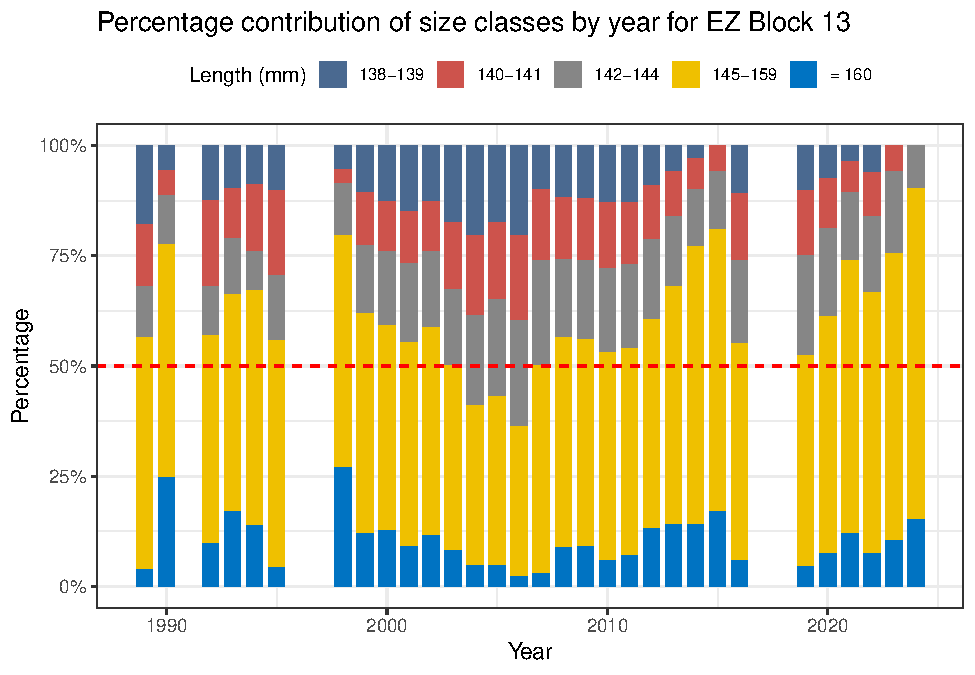
\includegraphics[width=0.8\textwidth,height=0.8\textwidth]{MM_Length-Weight_LML_files/figure-latex/size contribution plot-1} \end{center}

\section{Conclusions - these are just notes from various emails thus
far}\label{conclusions---these-are-just-notes-from-various-emails-thus-far}

Animals have mostly come from a fairly narrow band 138-150 mm; there are
certainly not too many large cohorts remaining above 160 mm however
there are evidence of large animals existing so if given a chance to
grow they would attain larger max size.

Exploitation rate is too high (still) in the Eastern Zone, so it remains
something of a recruit based fishery. Thus, any external events (storms,
MHW, crap year ), means that the harvest has to switch to larger size
classes (\textgreater{} 145mm) of which there is not much, and CPUE
falls quickly.

DOES NOT support the idea that the growth in these populations is
limiting and that something like a 145mm size limit is to high.

About 70\% of catch is \textless150 mm and the data points to a reliance
on very much a recruit-based fishery, where individuals are taken as
soon as they enter the fishery, and larger cohorts have effectively been
picked off gradually over the years to the point that when the fishery
does need to shift to bigger fish (i.e.~now) they simply aren't there or
have never had the chance to reach those larger sizes.

\section{References}\label{references}

\end{document}
